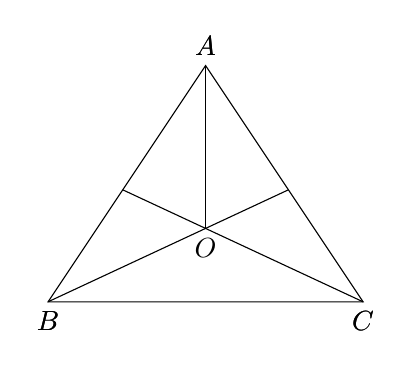
\begin{tikzpicture} 
        \coordinate (A) at (2, 3) {};
        \coordinate (B) at (0, 0) {};
        \coordinate (C) at (4, 0) {};
        \coordinate (O) at (2, 0.93) {};
        \coordinate (B1) at (3.051863, 1.422205) {};
        \coordinate (B2) at (0.9481367, 1.422205) {};
        \draw (A)node[above]{$A$}--(B)node[below]{$B$}--(C)node[below]{$C$}--cycle;
\draw (A)node[above]{$A$}--(O)node[below]{$O$};
\draw (B)node[below]{$B$}--(B1)node[right]{};
\draw (C)node[below]{$C$}--(B2)node[left]{};
\tkzMarkSegments[mark=|,color=black,size=3pt](C,A A,B)
\end{tikzpicture}